\bexo
Tracer sur la même figure
\begin{itemize}
	\item $t\mapsto \sin(t)$
	\item $t\mapsto -2\cos(\frac{1}{2}x)$ avec $x=2t-\pi$
	\item $t\mapsto \frac{1}{2}\sin(2t)$
\end{itemize}

	\begin{center}
	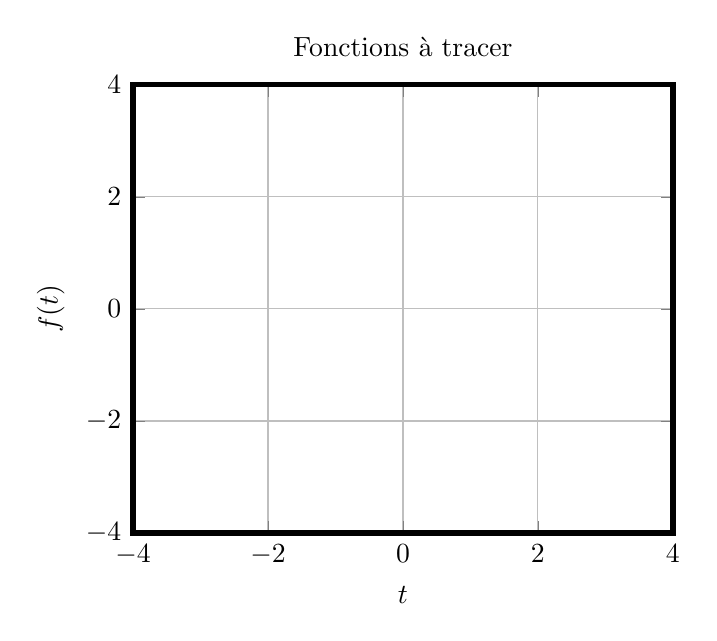
\begin{tikzpicture}
	  \begin{axis}[
				line width=2pt,
				legend columns=-1,
				title=Fonctions à tracer,
				xlabel={$t$},
				ylabel={$f(t)$},
				xmin=-4,
				xmax=4,
				ymin=-4,
				ymax=4,
				legend to name=named,
				grid=major]
	  \end{axis}

	\end{tikzpicture}
		  \ref{named}
\end{center}





\eexo
\solution{
Les graphes des fonctions sont:\\

	\begin{center}
	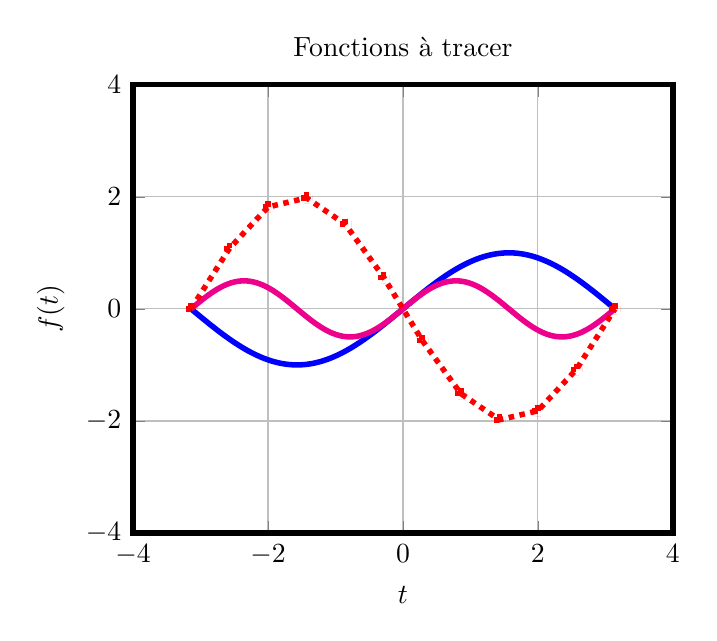
\begin{tikzpicture}
	  \begin{axis}[
				line width=2pt,
				legend columns=-1,
				title=Fonctions à tracer,
				xlabel={$t$},
				ylabel={$f(t)$},
				xmin=-4,
				xmax=4,
				ymin=-4,
				ymax=4,
				legend to name=named,
				legend entries={$\tr{sin}(t)$,$\frac{1}{2}\sin(2t)$,$-2\cos(\frac{1}{2}x)$},
				grid=major]
			\addplot[blue] expression[domain=-pi:pi,samples=500]{sin(180*x/pi)};
			\addplot[magenta,samples=500] expression[domain=-pi:pi]{0.5*sin(2*180*x/pi)};
			\addplot[dotted,red,mark=+,samples=12] expression[domain=-pi:pi]{-2*cos(180*x/pi-90)};
		\end{axis}
	\end{tikzpicture}
		  \ref{named}
\end{center}


}
